%!TEX root = ../main.tex
\chapter{RBM, IL-RBM}
本章では,提案システムを構成する主要なネットワークであるRestricted Boltzmann Bachine(RBM)\cite{RBM1,Hinton-guide ,fischer2012introduction}とIL-RBM\cite{osawa}について説明する.

\section{Restricted Boltzmann Machine}
\subsection{Restricted Boltzmann Machineの概要}
Restricted Boltzmann Machine(RBM)とは,1982年,J.J.Hopfieldが発表した\cite{hopfield1982neural}ホップフィールドネットワークの一種であるBoltzmann Machineの可視層間,隠れ層間の結合を制限したものである.
 
Boltzmann Machineは,連想記憶のモデルとして有力なニューラルネットワークであったが,学習時間が発散してしまうため,問題のサイズがある程度以上になると現実的に学習が不可能であるという欠点が存在した.

RBMはBoltzmann Machineの可視層間,隠れ層間の各ノードの結合を制限することで,学習時間を現実的な値まで減らしたモデルであり,後述するContrastive Divergence法\cite{CD}と呼ばれる洗練された学習方法の登場もあり,現在様々な分野で広く利用されているニューラルネットワークの一つである.

%その学習における結合の重みの変化の過程が,脳における神経科学的な学習則であるヘブ則とも類似しているなど,ニューラルネットワークの現在非常に有力な手法の一つである.

図\ref{fig:rbm}に示すように,RBMは可視層と隠れ層の二層で構成される.基本的なRBMでは,各ノードは0か1の値を取る(拡張されたRBMには実数値を扱えるRBMも存在する\cite{ackley1985learning}).

\begin{figure}[tb]
 \begin{center}
  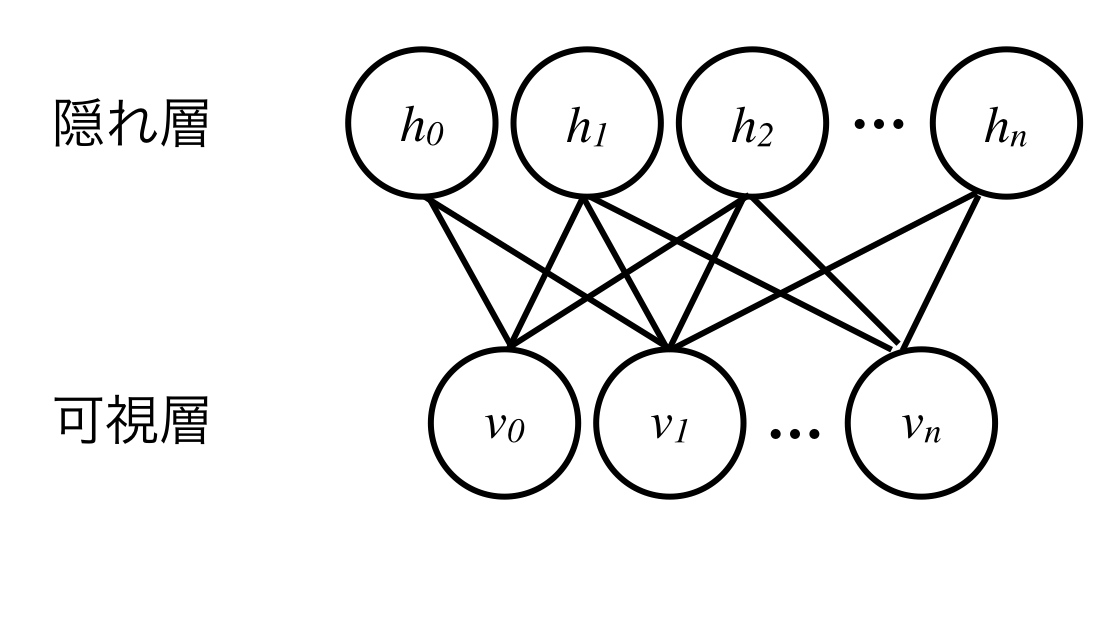
\includegraphics[scale=0.6]{./koki/rbm.png}
  \caption{Restricted Boltzmann Machine}
  % \ecaption{Representations of Data} 
  \label{fig:rbm}
 \end{center}
\end{figure}

可視層と隠れ層のノードの値を示すベクトルを以下のように定義する.

\begin{eqnarray}
	\bm{v} & = & (v_0,v_1,...v_{V-1} ), \forall v_i \in {0,1} \\
	\bm{h} & = & (h_0,h_1,...h_{H-1} ), \forall h_i \in {0,1}
\end{eqnarray}

この時,RBMでは可視層と隠れ層の結合確率が以下のように定義される.

\begin{eqnarray}
	p(\bm{v}, \bm{h}; \theta) & = & \frac{1}{Z(\theta)}  \exp (-E(\bm{v},\bm{h};\theta)) \label{fig:rbm_p}\\
	E(\bm{v}, \bm{h}; \theta) & = & -\sum_i b_i v_i - \sum_j c_j h_j- \sum_i \sum_j v_i W_{ij} h_j \label{fig:rbm_e}
\end{eqnarray}

ここで$b_i,c_j,W_{ij}$はそれぞれ可視素子 $v_i$ のバイアス,隠れ素子 $ h_j $ のバイアス,可視素子 $ v_i $ と隠れ素子 $ h_j $ の間のウェイトパラメータである.
これらのパラメータをまとめて $ \theta $ とする.
また $ Z $ は正規化定数であり,以下のように定義される.

\begin{equation}
	Z(\theta)= \sum_{\bm{v}} \sum_{\bm{h}} \exp (-E(\bm{v}, \bm{h}; \theta))
\end{equation}

式\ref{fig:rbm_p},式\ref{fig:rbm_e}より,片方の層の状態が入力された時,他方の層の各ノードの取る値の条件付き確率が計算できる.そのため,ある隠れ層の状態から入力を確率的に生成することが可能なため,RBMは生成モデルであるという側面を持つ.

RBMは,可視層に入力データを入れ学習させることで,隠れ層にその特徴をよく表すようなパラメータを出力することができる\cite{hinton2006reducing}.この特徴を用いて,後述するDeep Belief Netのように,ディープニューラルネットワークのプレトレーニングに用いられることも多い.

\subsection{RBMの学習}\label{sec:learn}
\subsubsection{計算の概略}
RBMの学習では,可視層の観測データ$\bm{v}$に対する$p(\bm{v})$について最尤推定を行う.

$p(\bm{v})$を計算するため結合確率 $p(\bm{v},\bm{h})$ を $\bm{h}$ について周辺化する.


\begin{eqnarray}
	p(\bm{v};\theta) & = & \sum_{\bm{h}} p(\bm{v},\bm{h};\theta) \\
				& = & \sum_{\bm{h}} \frac{1}{Z(\theta)} \exp (-E(\bm{v}, \bm{h}; \theta))
\end{eqnarray}

計算の簡単のため,以下では尤度の対数をとった対数尤度を取り扱う.

\begin{eqnarray}
	J & = & < \ln p(\bm{v}; \theta) >_q \\
	  & = & < \ln \sum_{\bm{h}} p(\bm{v}, \bm{h}; \theta) >_q \\
	  & = & < \ln \sum_{\bm{h}} \exp (-E(\bm{v}, \bm{h}; \theta) >_q - \ln Z(\theta) \\
	\theta ^* & = & \argmax_\theta  J
\end{eqnarray}

ここで $<>_q$ は確率分布 $q(\bm{v})$ の期待値を表す.

\begin{equation}
	<f(\bm{v})>_q= \sum_{\bm{v}} f(\bm{v}) q(\bm{v})
\end{equation}

また,$q(\bm{v})$ は観測データに関しての確率分布である.

\begin{equation}
	q(\bm{v}) = \frac{1}{N_{data}} \sum_n \delta(\bm{v}-\bm{v}^n)
\end{equation}

ここで$\bm{v}^k$は$k$番目の観測データを,
$ \delta(x)$は以下のように定義される関数である.

\begin{eqnarray}
\delta(x) = \begin{cases}
    1 & (n=0) \\
    0 & (otherwise)
  \end{cases}
\end{eqnarray}

ここで,対数尤度をパラメータ $ \theta $ について微分する.

\begin{eqnarray}
\frac {\partial J(\theta)}{\partial \theta} & = & 
	-<\frac{1}{\sum_{\bm{h}} \exp (-E(\bm{v}, \bm{h}; \theta))} 
	\sum_{\bm{h}} \frac{\partial E(\bm{v},\bm{h};\theta)}{\partial \theta} \exp(-E(\bm{v},\bm{h};\theta)) >_{q} \nonumber \\
	& & + \frac{1}{Z(\theta)} \sum_{\bm{v}} \sum_{\bm{h}} \frac{\partial E(\bm{v},\bm{h};\theta)}{ \partial \theta} \exp(-E(\bm{v},\bm{h};\theta))
\\
	& = & - \sum_{\bm{v}} \sum_{\bm{h}} \frac{\partial E(\bm{v},\bm{h};\theta)}{\partial \theta}
	\frac{\exp (-E(\bm{v},\bm{h};\theta)}{\sum_{\bm{h}} \exp(-E(\bm{v},\bm{h};\theta))} q(v) \nonumber \\
	& & + \frac{1}{Z(\theta)} \sum_{\bm{v}} \sum_{\bm{h}} \frac{\partial E(\bm{v},\bm{h};\theta)}{ \partial \theta} \exp(-E(\bm{v},\bm{h};\theta))
\\
	& = & < \frac{\partial E(\bm{v},\bm{h};\theta)}{ \partial \theta} >_{data}
	 - <\frac{\partial E(\bm{v},\bm{h};\theta)}{ \partial \theta} >_{model}
	 \label{eqa:pos_neg}
\end{eqnarray}

ここで,$<>_{data}$,$<>_{model}$はそれぞれ$p_{data}(\bm{v},\bm{h})=p(\bm{h}|\bm{v})q(\bm{v})$と$p_{model}(\bm{v},\bm{h})=p(\bm{v},\bm{h})$に対する期待値を表す.

ここで,第一項に関しては,可視層の状態から隠れ層の条件付き確率の厳密解が用意に計算できることから,計算はかなり容易である.一方,第二項に関しては,全ての$\bm{v}$,$\bm{h}$の組み合わせを計算しなければいけないため計算量が指数的に爆発してしまう.

したがって第二項を計算するため, サンプリング的手法や,近似的に解を求める手法などが用いられてきた.現在では次節で説明するContrastive Divergence法と呼ばれるサンプリング手法が最も有力であり,広く用いられている.

\subsubsection{Contrastive Divergence法}
Contrastive Divergence法(CD法)は,2002年にHintonによって発表されたRBMの学習におけるサンプリング手法である\cite{CD}.

厳密な$p(\bm{v},\bm{h})$を計算する代わりに,\bm{v}と\bm{h}をサンプリングして,$p(\bm{v},\bm{h})$を近似的に求める手法であるが,従来のギブスサンプリングとは遷移回数と可視層の初期値の選び方の点で異なる.

CD法では,\bm{v}と\bm{h}をサンプリングする際の可視層の初期値に,実際の観測データを用いる.RBMでは,各層のノードの取る値の条件付き確率は,他方の層のノードの状態にのみ依存しており,その確率はロジスティック関数

\begin{eqnarray}
  \sigma(x)= \frac{1}{1 + \exp(-x)}  
 \end{eqnarray}

を用いて

\begin{eqnarray}
	p(v_i=1│\bm{h}) & = & \sigma(b_i+ \sum_j W_{ij} h_j) \\
	p(h_i=1│\bm{v}) & = & \sigma(c_i+ \sum_i v_i W_{ij}) \\
	\sigma(x)		& = & \frac{1}{1 + \exp(-x)}
\end{eqnarray}

で表されるので,入力された可視層から隠れ層の状態を求めることができる.その後,同じように求めた隠れ層の状態から可視層の状態を計算可能である.

ギブスサンプリングでは,この可視層と隠れ層の間の遷移を通常多数回行う必要があったが,CD方では少ない回数でも上手く学習が進むことが経験的に知られており,多くの場合では遷移回数が1回でも十分である\cite{Hinton-guide,Bengio-AI,CD}.

このようにして得られた可視層の状態と条件付き確率より結合確率

\begin{eqnarray}
	p_{model}(\bm{v},\bm{h})=\frac{1}{N} \sum_k \delta( \bm{v} - \bm{v}_k ) p(\bm{h}|\bm{v}_k)
\end{eqnarray}

を求め,近似的に式(\ref{eqa:pos_neg})の第二項を求める.

\section{Deep Belief Net}

ディープニューラルネットワークを教師あり学習させようとした場合,過学習や局値解に陥ってしまうと言った問題が起きることがある.
このような問題を解決するためにプレトレーニングが行われることがあるが,プレトレーニングに前述したRBMの学習を用いたものをDeep Belief Net(DBN)\cite{DBN}という.

\begin{figure}[tb]
 \begin{center}
  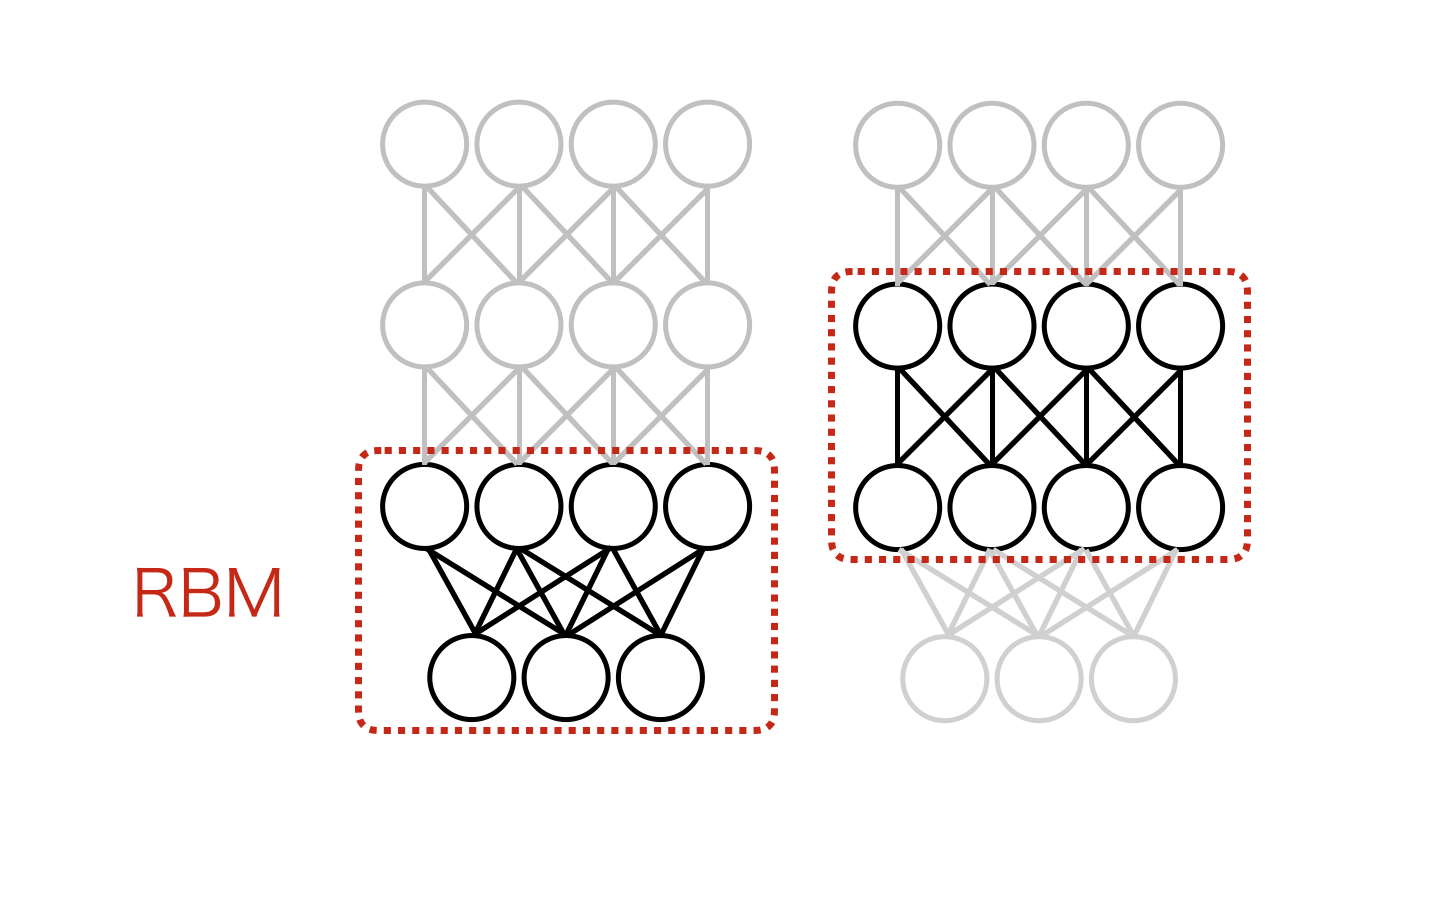
\includegraphics[scale=0.55]{./koki/dbn.png}
  \hspace*{0cm}
  \vspace*{0cm} 
  \caption{DBN学習過程}
  % \ecaption{Representations of Data} でんぱ
  \label{fig:dbn}
 \end{center}
\end{figure}

図\ref{fig:dbn}にプレトレーニング\cite{glw-training}の手順を示す.

まず,ディープニューラルネットワークの第一層と第二層をRBMとみなしRBMの学習を行う.可視層に入力した入力データの特徴の表現が隠れ層に表れるというRBMの利点を,ディープニューラルネットワークのプレトレーニングに活用する.

第一層と第二層にて学習を終えた後,このRBMの重みを固定し,入力データを伝播させて表れた隠れ層の状態を新たな入力データとして,第二層と第三層を新たなRBMとみなし学習を行う.

このように連鎖的に下層から上層に向かい二層ずつRBMとみなして教師なし学習を行い,出力層では教師あり学習を行う.

このようにプレトレーニングを終えた後,ネットワーク全体で誤差逆伝播法にて教師あり学習を行う手法もしばしば用いられ,これをファインチューニングと呼ぶ.

\section{Incremental Learning-RBM(IL-RBM)}\label{sec:rbm}

IL-RBM\cite{osawa}は追加学習を行うと既学習情報を失うというRBMの欠点を改良したものであり,追加学習を行う際に隠れ層の素子数を追加するという特徴がある.
追加する素子数を学習データセットを考慮し自動で決定するアルゴリズムと,ネットワークのエネルギーより既学習データと未学習データを判別するアルゴリズムも同時に説明する.

\subsection{隠れ層ノード数の自動決定法}\label{sec:node}
RBMの隠れ層のノード数の自動決定を行うアルゴリズムについて説明する.文献\cite{osawa}において,図\ref{fig:pre_exp_line}\footnote{大澤正彦,萩原将文:"RBMにおける未学習データ検出法の提案と追加学習への応用" vol.114, no.259, NC2014-118, pp.283-288, 2015-3.より引用}に示すように,学習済みRBMのクロスエントロピーと隠れ層ノード数には以下の関係が有ることが述べられている.

\begin{itemize}
 \item  隠れ層のノード数が非常に少ない場合,ノード数にかかわらずクロスエントロピーが一定である領域が存在する場合がある.
  \item 隠れ層のノード数が不十分な場合,隠れ層のノード数を増やした際に学習済みRBMのクロスエントロピーは一般に減少し,その減少は線形に近似することができる.
  \item 隠れ層ノード数が十分な値に達した場合,隠れ層のノード数を増やしても学習済みRBMのクロスエントロピーは減少しない.  
\end{itemize}

\begin{figure}[]
\begin{center}
   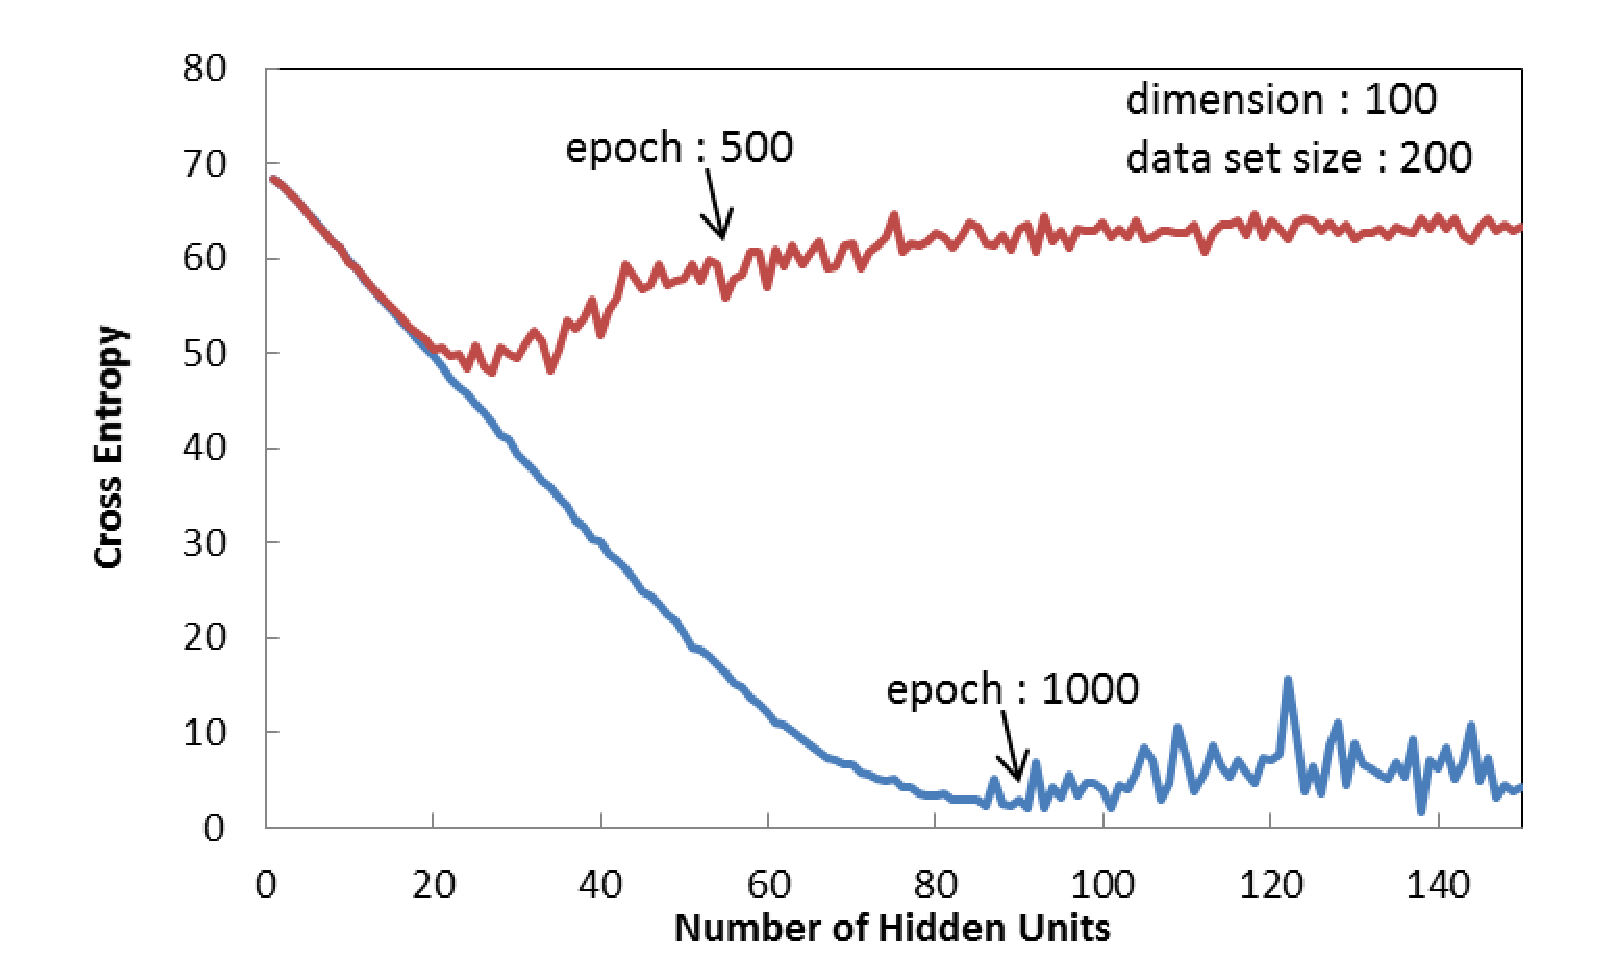
\includegraphics[scale=0.58]{./myimg/pre_exp1_c.eps} \\
   \caption{隠れ層ノード数とクロスエントロピーの関係}
  \label{fig:pre_exp_line}
\end{center}
\end{figure}

この関係を用いて,文献\cite{osawa}にてRBMの素子数の自動決定法が提案されている.

RBMの素子数の自動決定法は傾斜検出フェーズと傾斜予測フェーズの2つのフェーズに分けることができる.

\subsubsection{傾斜検出フェーズ}
傾斜検出フェーズは,ニューロン数にかかわらずクロスエントロピーの変化しない領域をスキップし,傾斜の始まりを正しく検出するためのフェーズである.図\ref{fig:phase1}\footnote{大澤正彦,萩原将文:"RBMにおける未学習データ検出法の提案と追加学習への応用" vol.114, no.259, NC2014-118, pp.283-288, 2015-3.より引用}に傾斜検出フェーズの実行過程を示す.

\begin{figure}[]
\begin{center}
  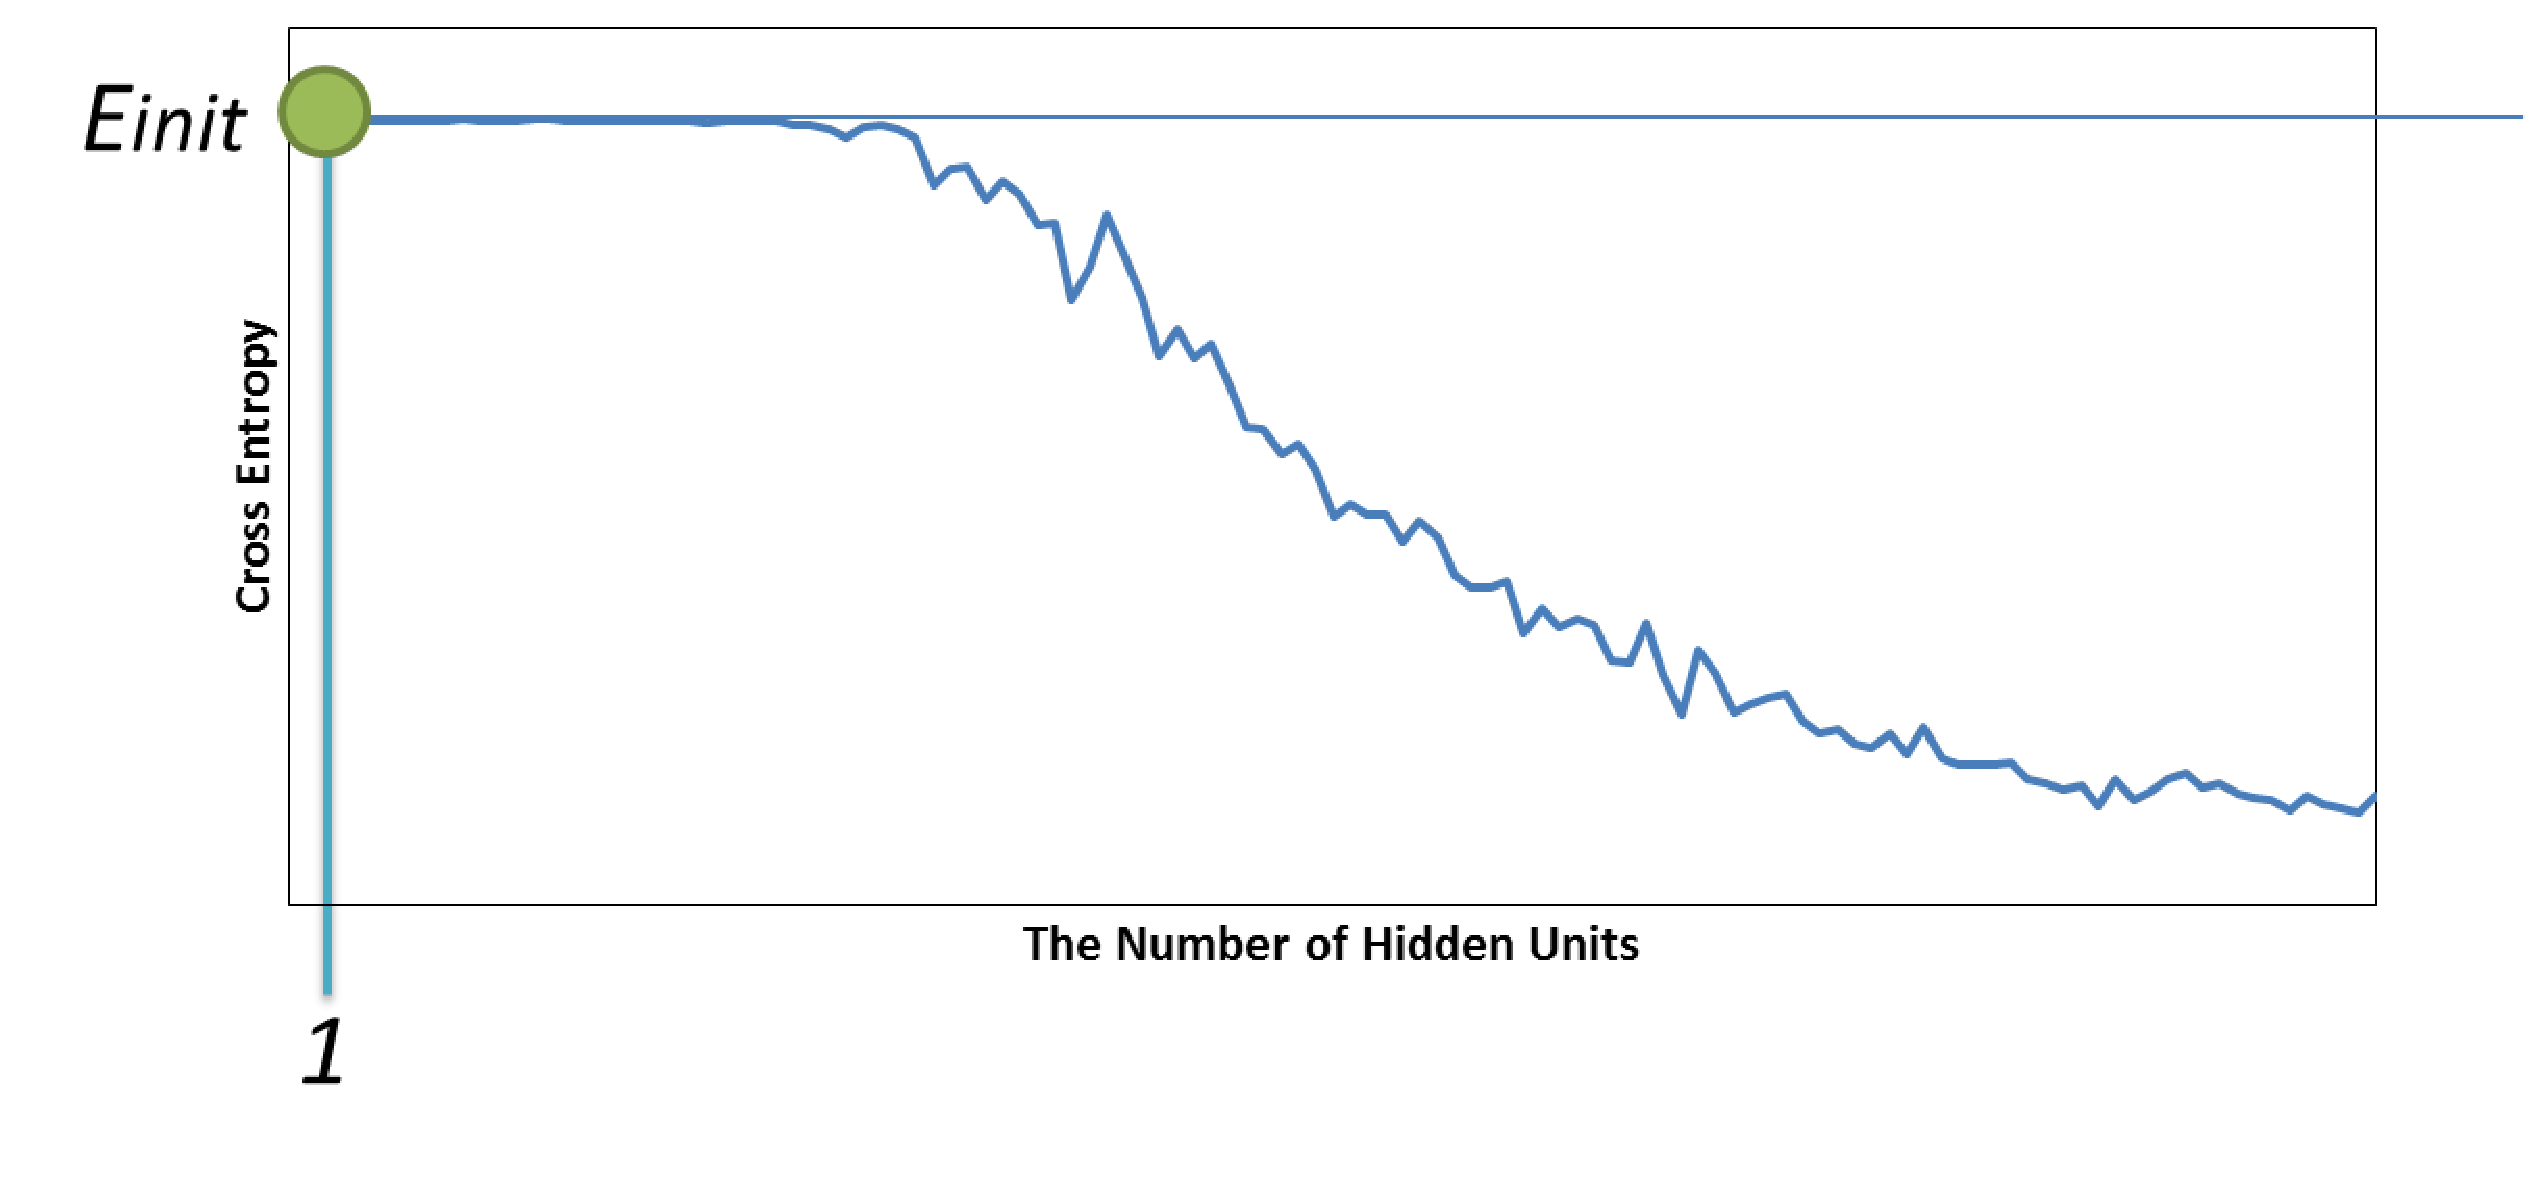
\includegraphics[scale=0.34]{./myimg/phase1_1.eps} \\
  (a) $E_{init}$の決定 \\
  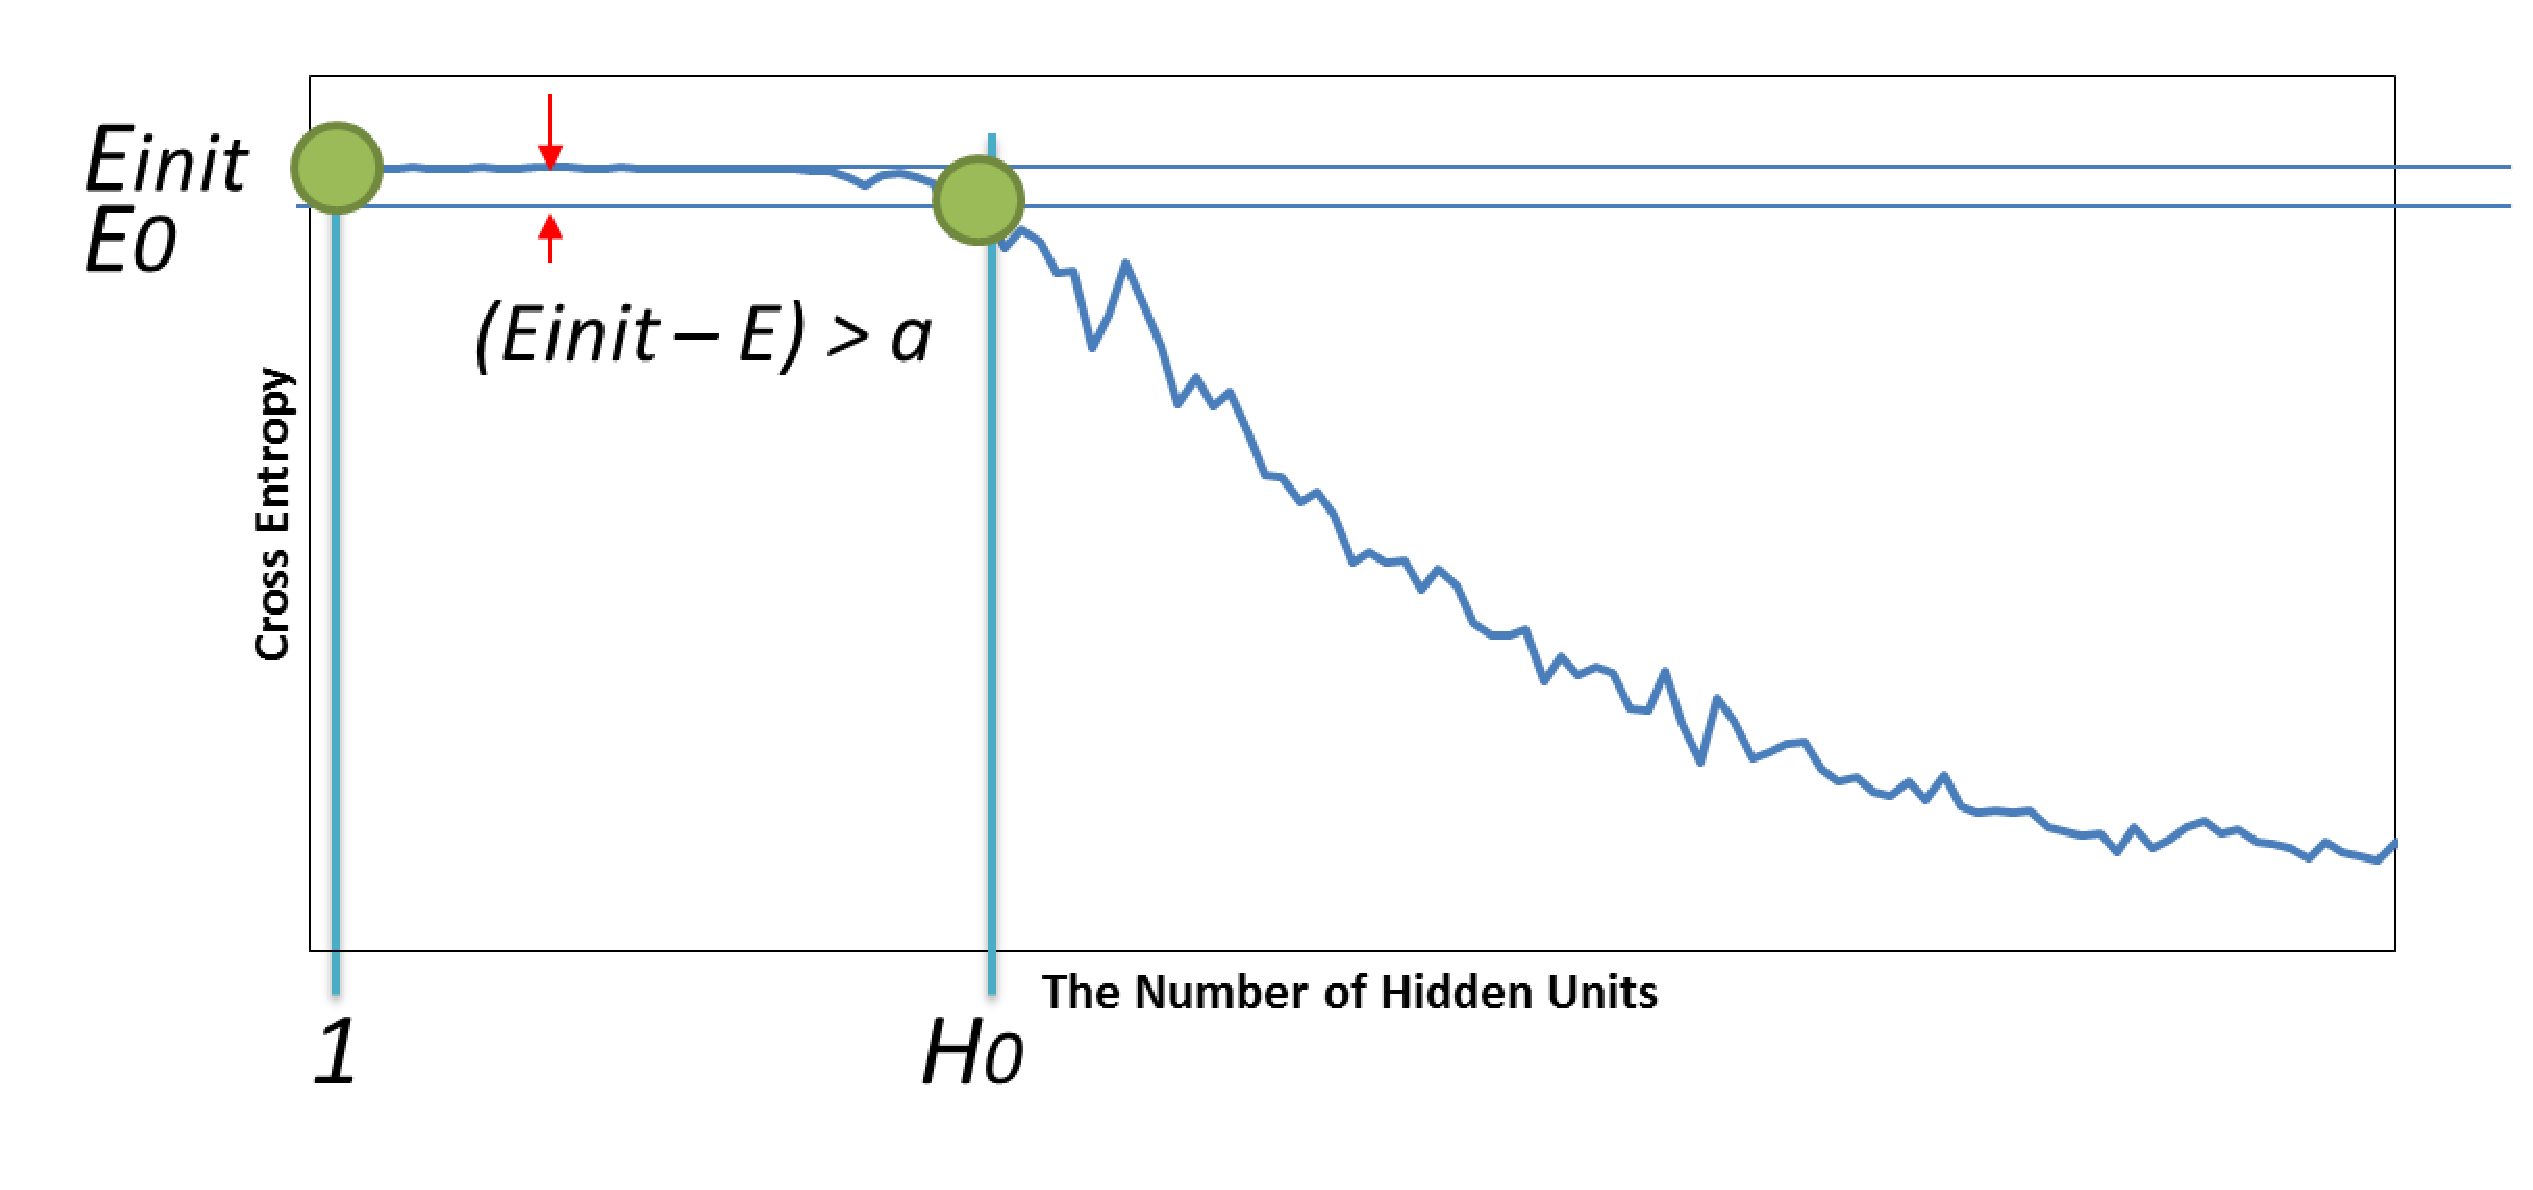
\includegraphics[scale=0.34]{./myimg/phase1_3.eps} \\
  (b) 閾値$a$との比較 \\
  \caption{傾斜検出フェーズの実行過程}
  % \ecaption{An Execution Process of Phase1}
  \label{fig:phase1}
\end{center}
\end{figure}

ニューロン数が1の時のクロスエントロピーを$E_{init}$と置く.その後,ノード数を増加させつつサンプリングしたクロスエントロピーと$E_{init}$との差がある閾値を超えた場合にクロスエントロピーの減少が始まったと判断し,その点を傾斜の開始とみなす.

傾斜の開始を検知した後,ノード数をいくつかサンプリングしてクロスエントロピーを求める.サンプリングした点から傾斜の傾きを計算し,クロスエントロピーの減少を線形で近似する.

最終的な隠れ層のノード数は,クロスエントロピーの近似式の値が0となる時のノード数が選ばれる.

\subsection{追加学習}
II-RBMでは追加学習を行う.追加学習とは,既にあるデータセットに対し学習済みのニューラルネットワークが,新たなデータセットに対し,既学習情報を失わない形で学習を行うことである.既にあるデータセットで学習したRBMの重みを変更しないように新たなデータセットに対して学習を行う.

通常のRBMの隠れ層のノード数は一定である.しかし,IL-RBMは新たなデータセットを学習する際に隠れ層のノード数を追加する操作を行う.

図\ref{fig:ilrbm}に示すようにIL-RBMの学習は次のような流れをとる.

\begin{figure}[tb]
 \begin{center}
  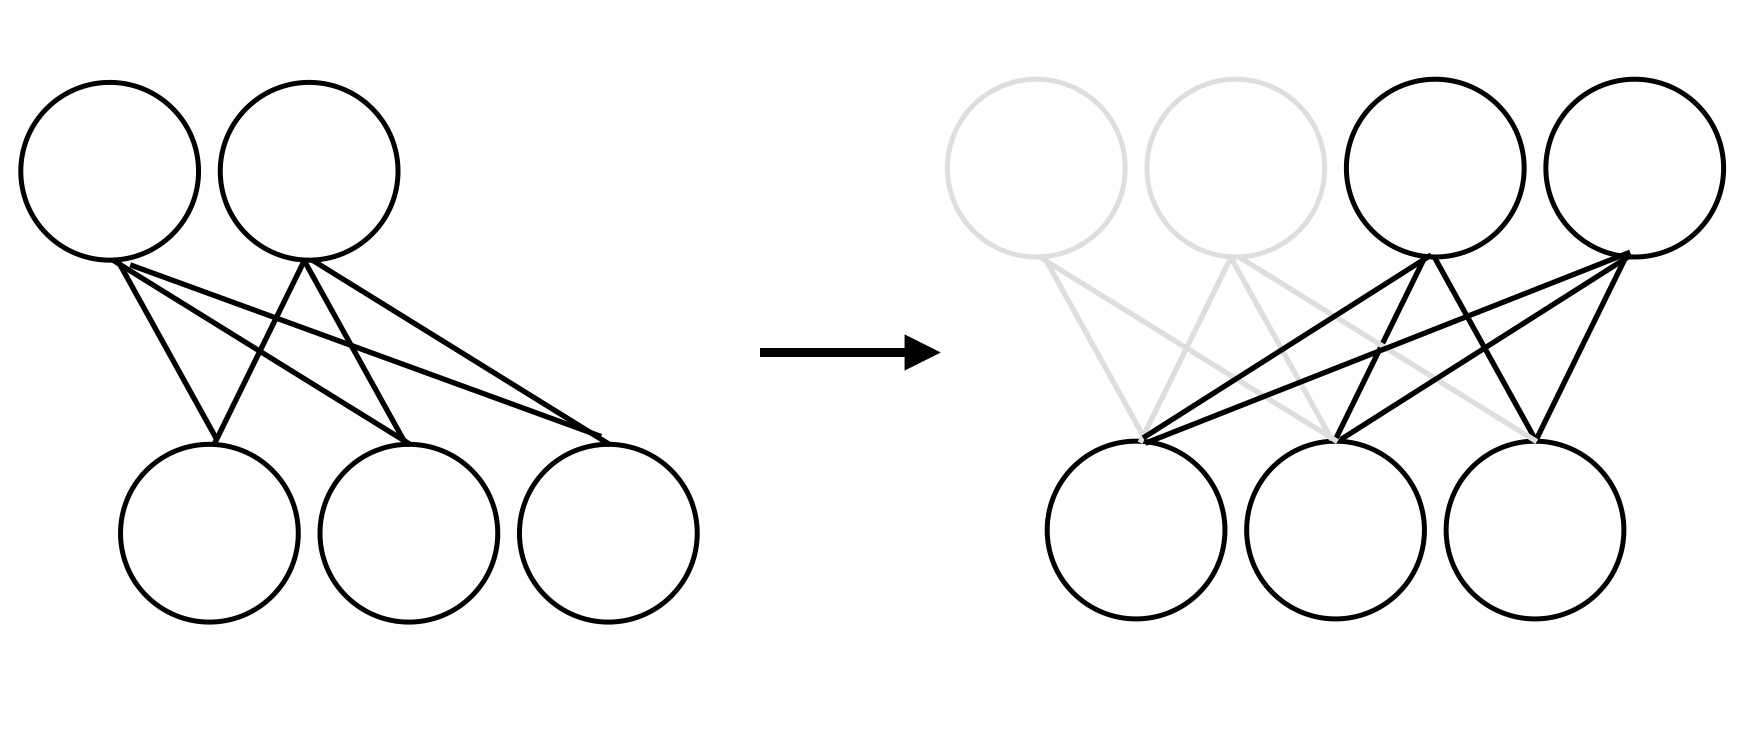
\includegraphics[scale=0.5]{./koki/ilrbm.png}
  \hspace*{0cm}
  \vspace*{0cm} 
  \caption{IL-RBM素子追加過程}
  \label{fig:ilrbm}
 \end{center}
\end{figure}

\begin{enumerate}
  \item 初期データセットに対しIL-RBMを学習させる.
  \item 追加データセットに対し,適切な追加ノード数を決定し,Il-RBMの隠れ層にノードを追加する.
  \item 上記手順で追加したノードのみを用いて,追加データセットを学習させる.
  \item 上記2,3の手順を追加データセットの分だけ繰り返し行う.
\end{enumerate}

追加データセットに対する適切な追加ノード数の決定には\ref{sec:node}節で説明したノード数の自動決定法を用いる.